\section{Method}
\label{sec:method}

\begin{figure}[t]
\centering
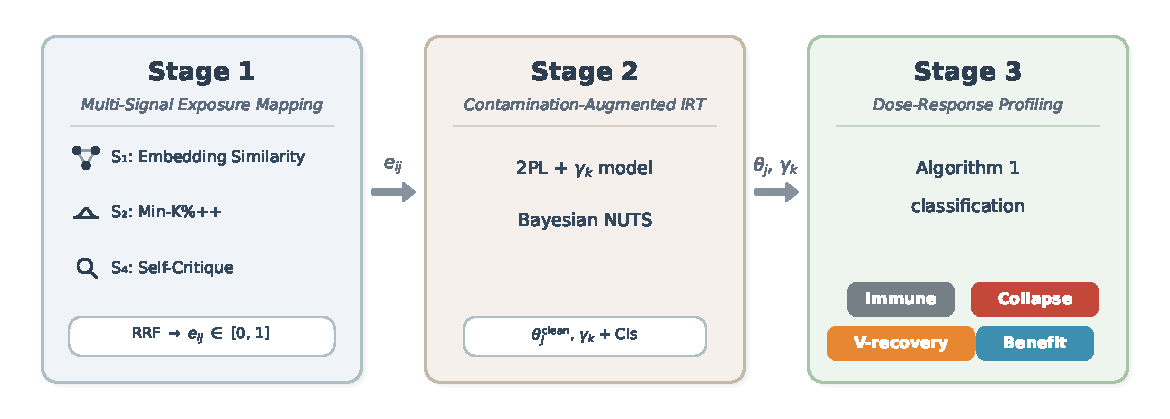
\includegraphics[width=\columnwidth]{figures/fig_pipeline.pdf}
\caption{ContamCal three-stage pipeline. Stage~1 fuses training-free detection signals into per-item exposure scores via Reciprocal Rank Fusion. Stage~2 embeds these scores in a contamination-augmented 2PL IRT model, recovering clean ability estimates with credible intervals. Stage~3 classifies the resulting dose-response trajectories into canonical patterns.}
\label{fig:pipeline}
\end{figure}

ContamCal operates in three stages (Figure~\ref{fig:pipeline}): Stage~1 estimates per-item contamination exposure via training-free signal fusion; Stage~2 embeds these scores in a contamination-augmented IRT model to recover clean ability estimates with credible intervals; Stage~3 classifies dose-response trajectories into canonical patterns.

\subsection{Problem Formulation}
\label{sec:formulation}

Let $y_{ijk} \in \{0,1\}$ denote the binary response of model~$j$ ($j=1,\ldots,J$) to item~$i$ ($i=1,\ldots,I_k$) on benchmark~$k$. Standard IRT assumes $P(y_{ijk}=1) = f(\theta_j, \boldsymbol{\xi}_i)$ where $\theta_j$ is latent ability and $\boldsymbol{\xi}_i$ collects item parameters. When training corpora contain benchmark items, the observed ability $\hat{\theta}_j$ confounds genuine capability with memorization.

Our goal is to estimate $\theta_j^{\text{clean}}$, the ability each model would exhibit absent contamination, and to diagnose contamination effects at domain granularity. We adapt item compromise IRT \citep{eckerly_2017_item_compromise,sinharay_2017_preknowledge} and explanatory IRT \citep{deboeck_2004_explanatory_irt} for LLM evaluation: replacing binary leakage indicators with continuous exposure scores $e_{ij} \in [0,1]$, fitting per-benchmark models to handle the shared item pool \citep{de_ayala_2009_irt}, and recovering clean ability via counterfactual inference (setting $e_{ij}=0$).

\subsection{Stage 1: Multi-Signal Exposure Mapping}
\label{sec:stage1}

For each model~$j$ and item~$i$, we consider four candidate detection signals. \textbf{S1}~(Embedding similarity): cosine similarity between the item embedding and its nearest neighbor in the SFT training corpus. \textbf{S2}~(Min-K\%++): a membership inference statistic based on token-level surprisal \citep{zhang_2024_minkpp}. \textbf{S3}~(ConStat): the accuracy gap between original and paraphrased item variants \citep{dekoninck2024constat}. \textbf{S4}~(Self-Critique): negative entropy of model self-evaluation distributions, inspired by the finding that LLMs can assess their own knowledge \citep{kadavath2022}; concurrent work by \citet{tao2025detecting} uses a related but mechanistically distinct entropy collapse approach targeting RL-trained models. S3 requires paired paraphrased items as reference and is therefore limited to benchmarks with existing paraphrase sets. Our primary pipeline uses the remaining three signals ($\mathcal{S} = \{\text{S1, S2, S4}\}$) and applies to any benchmark without auxiliary data. S2 and S4 exhibit known failure modes under RL post-training, which we characterize in \S\ref{sec:signal_failure}. Item-level classification performance of the exposure scores is reported in Appendix~\ref{sec:sij_classification}.

We aggregate signals via Reciprocal Rank Fusion \citep[RRF;][]{cormack_2009_rrf}:
\begin{equation}
\label{eq:rrf}
    e_{ij} = \sum_{s \in \mathcal{S}} \frac{1}{\kappa + r_{s}(i)},
\end{equation}
where $r_s(i)$ is the rank of item~$i$ under signal~$s$ (rank~1 = most suspicious), $\kappa=60$ is the standard RRF smoothing constant, robust to near-random component signals, and $|\mathcal{S}|=3$ in our primary configuration. Raw scores are min-max normalized per model to $e_{ij} \in [0,1]$; the distribution is highly right-skewed (mean 0.041).

\subsection{Stage 2: Contamination-Augmented IRT}
\label{sec:stage2}

\paragraph{Primary model: 2PL+$\gamma$.}
Our primary specification augments the two-parameter logistic (2PL) model \citep{lord_1980_irt,hambleton_1991_irt} with a contamination covariate. We fit independent IRT models per benchmark~$k$, each with its own contamination effect $\gamma_k$. Per-benchmark fitting avoids cross-benchmark item parameter borrowing while permitting heterogeneous contamination effects. For benchmark~$k$, the response probability is:
\begin{equation}
\label{eq:2pl_gamma}
    P(y_{ijk} = 1) = \sigma\!\bigl(a_i(\theta_j - b_i) + \gamma_k \cdot e_{ij}\bigr),
\end{equation}
where $\sigma(\cdot)$ is the logistic function, $a_i > 0$ is item discrimination, $b_i \in \mathbb{R}$ is item difficulty, $\theta_j$ is model ability, and $\gamma_k$ is the scalar contamination effect for benchmark~$k$ ($\gamma$ without subscript denotes the pooled effect; $\gamma_d$ denotes per-domain effects, \S\ref{sec:domain_differential}). Each benchmark is fitted independently; when finer-grained diagnosis is needed, we replace $\gamma_k$ with per-domain effects $\gamma_d$ ($d=1,\ldots,D$), fitting Eq.~\eqref{eq:2pl_gamma} separately for each cognitive domain within a benchmark (\S\ref{sec:domain_differential}).

We place $\gamma_k$ outside the item discrimination bracket, modeling contamination as a fixed logit shift \citep{de_ayala_2009_irt} rather than the uniform DIF form that would scale contamination effects with item discrimination. A comparison with the uniform DIF alternative ($\gamma$ inside the discrimination bracket) yields equivalent model fit (Appendix~\ref{sec:dif_comparison}). For MC-format benchmarks, a 4PL extension adds guessing and ceiling asymptotes (Appendix~\ref{sec:4pl_details}); this requires $J \geq 16$ and is not used in domain-level analyses ($J = 13$).

\paragraph{Inference.}
We perform Bayesian inference via NUTS \citep{hoffman2014} in Stan \citep{carpenter2017} with four chains and target acceptance 0.95. Priors: $\theta_j \sim \mathcal{N}(0,1)$, $a_i \sim \text{LogNormal}(0, 0.5)$, $b_i \sim \mathcal{N}(0,1)$, $\gamma_k \sim \mathcal{N}(0,1)$. At $J=16$, the $\gamma$ posterior is sensitive to the prior (up to 2.6$\times$ shift across reasonable alternatives; Appendix~\ref{sec:prior_sensitivity}); we therefore treat $\gamma$ estimates as directional indicators rather than precise effect sizes. Convergence requires split-$\hat{R} < 1.01$ and bulk ESS~$> 400$ for all parameters. Model fit is assessed via the posterior predictive $p$-value (PPP), where values near 0.5 indicate adequate fit.

\paragraph{Calibrated score.}
The decontaminated accuracy for model~$j$ on benchmark~$k$ is the posterior expectation under zero exposure:
\begin{equation}
\label{eq:calibrated}
    \text{Acc}_{j}^{\text{cal}} = \frac{1}{I_k} \sum_{i=1}^{I_k}\, \mathbb{E}_{\boldsymbol{\psi} \sim p(\boldsymbol{\psi} \mid \mathbf{y})} \!\left[\sigma\!\bigl(a_i(\theta_j - b_i)\bigr)\right],
\end{equation}
with credible intervals from posterior quantiles. In practice, we average $\sigma(a_i(\theta_j - b_i))$ over posterior draws with $e_{ij}=0$; the spread of draws yields the credible interval. Models with noisier exposure signals receive wider intervals by construction.

\paragraph{Identifiability.}
\label{sec:fisher}
\label{sec:value_decomposition}
The reliability of $\gamma$ depends on signal AUC and ensemble size $J$; simulation validates that recovery requires AUC$\geq$0.55 with $J \geq 50$ (Appendix~\ref{sec:identifiability_appendix}; DGP robustness in Appendix~\ref{sec:threshold_dgp}). Empirically, exposure scores $e_{ij}$ and item difficulty $b_i$ are near-orthogonal (Pearson $|r|<0.13$, $R^2<0.014$ across benchmarks), so $\gamma$ is identified from dosage-induced variation rather than confounded with difficulty. Eq.~\eqref{eq:calibrated} depends on $\theta_j$, not $\gamma$ directly, predicting that vanilla 2PL ($\gamma\!=\!0$) achieves comparable calibration to 2PL+$\gamma$, with $\gamma_k$ serving diagnosis rather than calibration (\S\ref{sec:calibration_results}).

\subsection{Dose-Response Profile Classification}
\label{sec:classification}

Independent of the IRT calibration pipeline, we classify dose-response profiles via a deterministic decision tree (Algorithm~\ref{alg:profile-classification} in Appendix~\ref{sec:classification_algorithm}) parameterized by noise threshold $\tau{=}2$\,pp and severity threshold $\sigma{=}5$\,pp, drawing on pharmacological dose-response modeling \citep{hill1910aggregation,ritz2015dose}. The tree branches on the end-to-end accuracy shift $\Delta{=}a_{100}{-}a_0$, mid-dosage minimum, and maximum mid-trajectory deviation to assign one of four patterns: \textsc{Immune}, \textsc{Collapse}, \textsc{V-recovery}, or \textsc{Benefit}. All thresholds are explicit and adjustable; a 30-combination $(\tau, \sigma)$ grid sweep confirms all families are stable (180/180 pairs; Appendix~\ref{sec:classification_sensitivity}). Family-level classification uses \emph{direction} as the primary criterion (\S\ref{sec:cross_seed}): Immune if the bootstrap CI of the cross-seed mean $\Delta$(d100) includes zero and $|\text{mean}~\Delta| < \tau$; Borderline if the CI includes zero but $|\text{mean}~\Delta| \geq \tau$; otherwise Harm/Benefit by sign. Parametric model selection (Appendix~\ref{sec:parametric_dr}) confirms these classifications for extreme effects but lacks power at $n\!=\!3$ seeds, motivating the rule-based approach.